\documentclass[10pt,twocolumn,letterpaper]{article}

% \usepackage[review]{cvpr}      % To produce the REVIEW version
\usepackage{cvpr}                % To produce the CAMERA-READY version
% \usepackage[pagenumbers]{cvpr} % To force page numbers, e.g. for an arXiv version

\usepackage{graphicx}
\usepackage{booktabs}
\usepackage{amsmath}
\usepackage{amssymb}
\usepackage{xcolor}
\definecolor{cvprblue}{rgb}{0.21,0.49,0.74}
\usepackage[pagebackref,breaklinks,colorlinks,allcolors=cvprblue]{hyperref}

\title{Video Object Removal and Inpainting for AIAA 3201 Project 3}
\author{Shuyu HE \and Ziyi GUO}
\date{}

\begin{document}
\maketitle

\begin{abstract}
We study video object removal and background restoration in dynamic scenes through a staged comparison between a transparent classical baseline and stronger modern components.
Our pipeline starts from object segmentation, sparse optical flow, temporal median borrowing, and \texttt{cv2.inpaint}, then replaces only the restoration backend with ProPainter to isolate the effect of the inpainting model under fixed masks.
On \texttt{bmx-trees}, \texttt{tennis}, and two self-recorded wild videos, this controlled replacement substantially improves qualitative restoration.
We then analyze a real failure case, \texttt{wild\_video2}, where incomplete masks rather than weak restoration are the dominant bottleneck.
A prompt-guided SAM~2 refinement stage improves this sequence by strengthening temporal mask coverage while keeping ProPainter fixed.
We further test two follow-up variants: multi-prompt SAM~2 fusion and a lightweight SD2 keyframe inpainting baseline.
The first produces little additional gain over single-prompt SAM~2, and the second is feasible but does not clearly outperform ProPainter.
The resulting project offers a reproducible baseline, a controlled backend comparison, a targeted failure-to-improvement study, and two supplemental experiments that clarify which extensions are actually useful.
\textbf{GitHub Repository:} \url{https://github.com/HHHHsy-code/CV_project_3}
\end{abstract}

\section{Introduction}
Video object removal aims to erase dynamic foreground objects while reconstructing a visually plausible and temporally coherent background.
This capability is relevant to scene cleanup, video editing, robotics, and downstream perception.
In practice, however, overall quality depends on at least two coupled components: accurate object masks and a strong restoration backend.
This project is therefore organized around controlled substitutions rather than a single monolithic system comparison.

We begin with a classical baseline that is easy to inspect stage by stage.
We then keep the removal masks fixed and replace only the restoration module with ProPainter, which yields a cleaner comparison between classical completion and modern video inpainting.
After that, we concentrate on one informative real-scene failure case and improve only the masks with prompt-guided SAM~2 propagation.
This lets us ask a sharper question: if the inpainting backend is held fixed, does better temporal masking alone explain the improvement?
Finally, we examine two follow-up extensions, namely multi-prompt SAM~2 fusion and a lightweight image-level diffusion baseline, to determine whether they add meaningful benefit beyond the main refinement branch.
Our contributions are therefore empirical and diagnostic rather than algorithmic.
First, we build a transparent baseline and a controlled Part~1-versus-Part~2 comparison that isolates the value of a stronger restoration backend.
Second, we turn \texttt{wild\_video2} into a failure-to-improvement case study and show that prompt-guided SAM~2 mask propagation resolves the main bottleneck while keeping the restoration model fixed.
Third, we report two honest supplemental results---multi-prompt SAM~2 fusion and SD2 keyframe inpainting---that clarify which extensions do \emph{not} deliver meaningful additional gains in our current setting.

\section{Related Work}
Modern video object removal depends on several subproblems: detecting the target object, segmenting it accurately, propagating masks across time, and restoring the hidden background.
For object localization and instance segmentation, two representative lines of work are region-based methods such as Mask R-CNN~\cite{he2017mask} and transformer-based detectors such as DETR~\cite{carion2020detr}.
Although our current implementation uses YOLOv8-seg as the practical detector, these works provide the broader context for modern object-centric mask generation.

For general-purpose interactive segmentation, Segment Anything (SAM)~\cite{kirillov2023sam} shows that promptable foundation segmentation models can generalize across diverse scenes.
SAM~2 extends this idea from static images to images and videos, making prompt-guided mask propagation practical for video object segmentation and editing workflows~\cite{ravi2024sam2}.
Related tracking-oriented work such as Tracking Anything with Decoupled Video Segmentation also highlights the importance of robust temporal mask propagation when the downstream task depends on accurate frame-wise target coverage~\cite{cheng2023tracking}.

For restoration, ProPainter~\cite{zhou2023propainter} is a strong recent video inpainting model that combines propagation and transformer components to improve temporal consistency and texture completion.
This is directly relevant to our project because it lets us hold the masks fixed and isolate the contribution of the restoration backend.
For evaluation context, the DAVIS benchmark remains a standard reference for video object segmentation experiments~\cite{perazzi2016davis}, even though raw DAVIS masks do not by themselves provide the clean-background ground truth required for direct object-removal PSNR or SSIM.

\section{Method}
\subsection{Part 1: Classical Baseline}
Our baseline follows a modular classical pipeline.
We first use YOLOv8-seg to generate category-aware instance masks for likely dynamic objects such as people, bicycles, and vehicles.
Because object detection alone is insufficient in scenes that contain static foreground objects, we further filter each instance by sparse Lucas-Kanade optical flow computed inside the predicted mask region.
For the $i$-th detected instance on frame $t$, let $P_{t,i}$ denote the pixel set inside the instance mask and let $u_t(p)$ be the sparse optical-flow vector at pixel $p$.
We define a motion score
\begin{equation}
  s_{t,i} = \frac{1}{|P_{t,i}|} \sum_{p \in P_{t,i}} \|u_t(p)\|_2,
\end{equation}
and keep the instance only when $s_{t,i} > \tau_{\text{motion}}$ for a fixed threshold $\tau_{\text{motion}}$.
The dynamic removal mask on frame $t$ is therefore
\begin{equation}
  M_t = \bigcup_i \mathbf{1}[s_{t,i} > \tau_{\text{motion}}] \, B_{t,i},
\end{equation}
where $B_{t,i}$ is the binary mask of instance $i$.
The resulting binary masks are then dilated and cleaned with connected-component filtering so that thin boundaries and fragmented regions are less likely to be missed during removal.
For background restoration, we first borrow pixels from nearby frames with a temporal median strategy and then apply \texttt{cv2.inpaint} as a fallback to close remaining holes.
If $\mathcal{N}(t)$ is a temporal neighborhood around frame $t$, the borrowed background estimate at pixel $p$ can be written as
\begin{equation}
  \hat{I}^{\,\text{med}}_t(p) = \operatorname{median}\{ I_k(p) \mid k \in \mathcal{N}(t),\ p \notin M_k \},
\end{equation}
which is then used as a first-pass fill before spatial inpainting handles residual gaps.
This baseline is deliberately simple and transparent: each stage can be inspected independently, which makes later failure analysis easier.

\subsection{Part 2: AI-driven Pipeline}
Our current Part 2 experiment uses a controlled setup: we reuse the masks produced by Part 1 and replace only the restoration stage with ProPainter~\cite{zhou2023propainter}.
This isolates the contribution of the video inpainting model and makes the qualitative comparison easier to interpret.
In this sense, Part 2 is not just ``a stronger model''; it is a controlled replacement of one subsystem inside the same overall pipeline.
We additionally refine a failure case on \texttt{wild\_video2} using prompt-guided SAM~2 propagation~\cite{ravi2024sam2} while keeping ProPainter fixed, which lets us attribute the remaining gain to better mask quality rather than a different restoration backend.

\subsection{Part 3: Failure-case Extension}
The current most informative failure case is \texttt{wild\_video2}, where the moving person is not consistently covered by the automatic mask generator in the baseline system.
This means the original failure is not caused by the inpainting backend itself; the object is simply never marked for removal in several frames.
We therefore introduce a targeted mask-improvement experiment based on prompt-guided SAM~2 propagation~\cite{ravi2024sam2}, and we use the resulting refined masks with the same ProPainter backend to measure whether better masks alone improve the final removal result.

Our current Part~3 therefore has one main branch and two supplemental checks.
The main branch uses a single prompt-guided SAM~2 propagation run to produce refined masks for \texttt{wild\_video2}, then reruns ProPainter with the improved masks.
The first supplemental check is an ablation on temporal prompting: instead of a single prompt frame, we run SAM~2 from multiple non-empty seed frames and merge the propagated masks with either union or majority voting.
This tests a concrete tracking-inspired hypothesis: perhaps the remaining failure is caused by over-reliance on one prompt frame rather than by the propagation model itself.
The second supplemental check is a keyframe-level diffusion restoration baseline on four hard frames, which lets us ask whether a lightweight image-level generator clearly outperforms ProPainter once the mask is already reasonably good.

\section{Experiments}
\subsection{Datasets}
We currently use four sequences:
\texttt{bmx-trees}, \texttt{tennis}, \texttt{wild\_video1}, and \texttt{wild\_video2}.
The first two are provided course sequences with mask annotations for baseline evaluation.
The latter two are self-recorded real-scene videos with a single walking person crossing a mostly fixed background.
An optional DAVIS subset~\cite{perazzi2016davis} remains a useful next source for additional mask evaluation.
If we need restoration metrics such as PSNR or SSIM, we must construct a synthetic masked-frame benchmark with known clean targets rather than relying on raw DAVIS object masks alone.

\subsection{Implementation Details}
All experiments were run on a remote GPU server with CUDA-enabled PyTorch environments.
The Part~1 baseline was executed in our local project environment, while ProPainter and SAM~2 were installed in separate conda environments to avoid dependency conflicts.
For the controlled Part~2 comparison, we used the masks already produced by the Part~1 pipeline and passed them directly to ProPainter.
For the \texttt{wild\_video2} refinement experiment, we automatically selected a seed frame from the original Part~1 masks, converted the selected mask into a prompt box, propagated the object through the video with SAM~2, and then reran ProPainter with the refined mask directory.
For the multi-prompt ablation, we repeated this procedure from three non-empty seed frames ($75$, $139$, and $152$) and merged the resulting binary mask directories with union and majority voting.
For the diffusion branch, we prepared a keyframe-editing workspace on frames $75$, $113$, $151$, and $189$ and ran a lightweight SD2-based image inpainting baseline on those frames.
We also prepared a heavier SDXL-based AttentiveEraser wrapper, but that heavier branch was not needed for the final project conclusion once the lighter baseline had already shown no clear advantage over ProPainter.
This staged setup was useful in practice because it let us diagnose whether failures came from poor restoration or from poor mask coverage.

\begin{table}[t]
  \centering
  \small
  \setlength{\tabcolsep}{4pt}
  \begin{tabular}{@{}p{0.12\linewidth}p{0.23\linewidth}p{0.21\linewidth}p{0.31\linewidth}@{}}
    \toprule
    Stage & Mask source & Restoration & Experimental role \\
    \midrule
    Part 1 & YOLOv8-seg + motion filtering & Median + OpenCV inpainting & Transparent classical baseline \\
    Part 2 & Part 1 masks & ProPainter & Controlled backend replacement \\
    Part 3A & Single-prompt SAM~2 & ProPainter & Main failure-case refinement on \texttt{wild\_video2} \\
    Part 3B & Multi-prompt SAM~2 / SD2 keyframes & ProPainter / SD2 & Supplemental ablation and exploratory baseline \\
    \bottomrule
  \end{tabular}
  \caption{Compact summary of the experimental branches. The table makes the controlled substitutions explicit: Part~2 changes the restoration backend, while Part~3 primarily changes mask quality.}
  \label{tab:experiment-branches}
\end{table}

\subsection{Metrics}
For mask quality, we report $J_M$ and $J_R$, which correspond to region similarity and recall-style mask coverage, together with mean precision for additional interpretation.
Concretely, if $M_t$ is the predicted mask and $G_t$ is the ground-truth mask on frame $t$, then the region similarity is the standard Jaccard index
\begin{equation}
  J(M_t, G_t) = \frac{|M_t \cap G_t|}{|M_t \cup G_t|}.
\end{equation}
These metrics are directly applicable to \texttt{bmx-trees} and \texttt{tennis}, where foreground mask annotations are available.
For restoration quality, PSNR and SSIM are only meaningful when a clean target frame exists.
Since our current wild-video experiments do not provide clean-background ground truth, the main restoration evidence in this draft is qualitative rather than pixel-wise.
For the \texttt{wild\_video2} failure case, we therefore use two lightweight summary statistics over a $T$-frame sequence:
\begin{equation}
  C = \frac{1}{T} \sum_{t=1}^{T} \mathbf{1}\!\left[\|M_t\|_0 > 0\right],
\end{equation}
which measures temporal coverage, and
\begin{equation}
  A = \frac{1}{T} \sum_{t=1}^{T} \frac{\|M_t\|_0}{HW},
\end{equation}
which measures the mean normalized mask area on frames of size $H \times W$.
These statistics do not replace GT-backed metrics, but they help quantify whether a refinement is more persistent over time or merely produces larger masks.

\subsection{Quantitative Results}
Figure~\ref{fig:benchmark-mask-metrics} reports the current Part 1 mask quality results.
The two provided benchmark sequences exhibit different failure modes.
On \texttt{bmx-trees}, the baseline achieves high recall but low precision, which matches the visual observation that the masks are often too large and include extra background regions.
On \texttt{tennis}, the masks are much tighter, yielding a considerably stronger baseline for the later restoration comparison.
This difference in baseline mask quality is useful for interpretation: when ProPainter improves both sequences despite very different mask precision, the gain is more plausibly attributed to the restoration backend than to a trivial change in mask shape alone.

\begin{figure}[t]
  \centering
  \IfFileExists{assets/benchmark_mask_metrics.png}{
    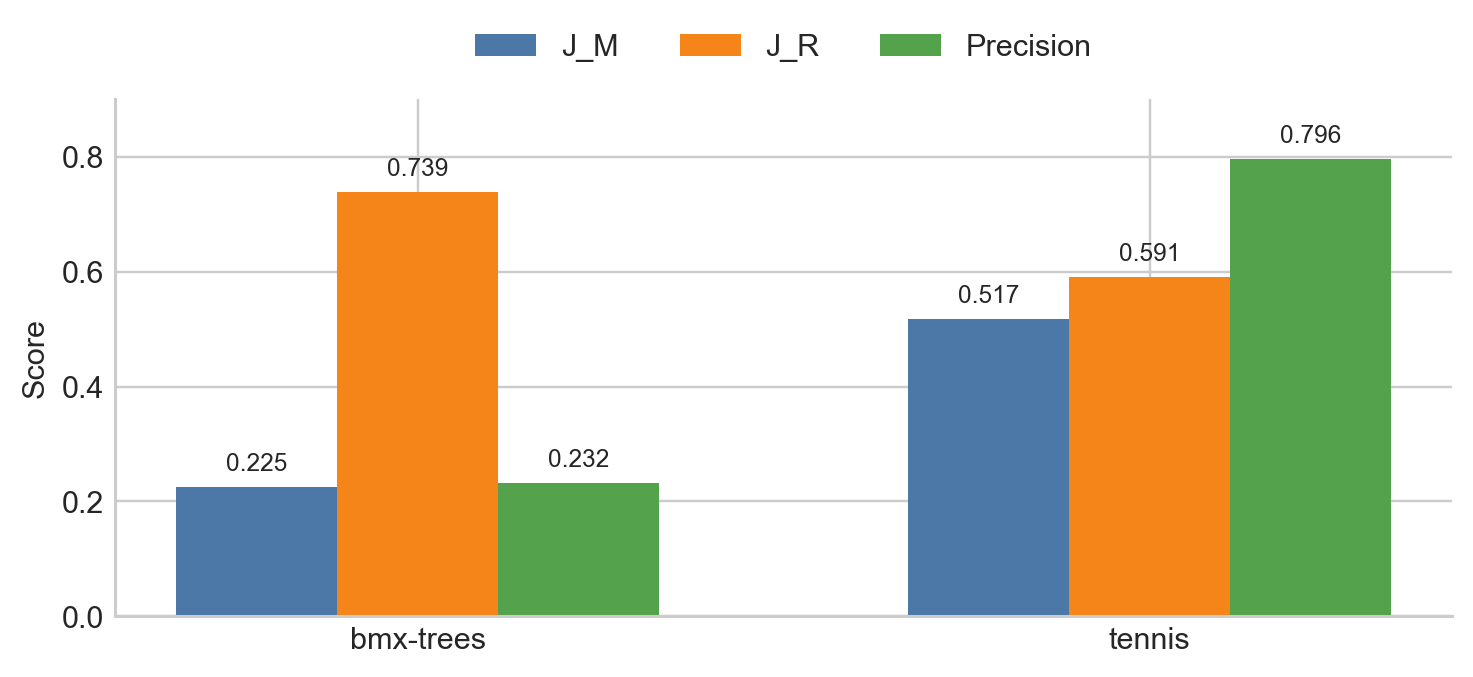
\includegraphics[width=\linewidth]{assets/benchmark_mask_metrics.png}
  }{
    \fbox{\rule{0pt}{1.5in}\rule{0.95\linewidth}{0pt}}
  }
  \caption{Benchmark mask quality on the two annotated course sequences. The contrast is informative: \texttt{bmx-trees} shows high recall but poor precision, while \texttt{tennis} is much more balanced and precise.}
  \label{fig:benchmark-mask-metrics}
\end{figure}

At the current project stage, the restoration story is best supported by controlled qualitative comparison rather than PSNR or SSIM.
Specifically, we keep the removal masks fixed and compare the classical temporal restoration module against ProPainter.
This design removes mask quality as a confounder and lets us isolate the benefit of a stronger video completion backend.
As a lightweight additional experiment, we also prepared a temporal mask-summary tool for the \texttt{wild\_video2} failure case.
This lets us compare how many frames contain a non-empty target mask before and after SAM~2 refinement, together with mean mask area ratio.
Although this is not a replacement for full GT-backed metrics, it provides a compact quantitative check that the refined masks are more temporally stable than the original automatic masks.
For \texttt{wild\_video2}, SAM~2 refinement increases temporal mask coverage from $0.547$ to $0.642$ and raises the number of non-empty mask frames from $104$ to $122$.
At the same time, the mean mask area ratio drops from $0.0166$ to $0.0115$, indicating that the improved masks are not simply larger; instead, they are more temporally stable and spatially tighter around the walking person.
Figure~\ref{fig:wild-ablation-metrics} summarizes the \texttt{wild\_video2} mask-side refinement results.
Compared with the original Part 1 masks, single-prompt SAM~2 increases temporal coverage from $0.547$ to $0.642$ and raises the number of non-empty mask frames from $104$ to $122$.
At the same time, the mean mask area ratio drops from $0.0166$ to $0.0115$, indicating that the refined masks are not merely larger; they are also spatially tighter.
However, the multi-prompt ablation shows that simple prompt ensembling does not further improve this sequence: both union and majority-vote fusion produce almost identical temporal coverage and area statistics.
This negative result is useful because it narrows the interpretation of the remaining error: the main gain comes from moving from weak automatic masks to prompt-guided SAM~2 propagation, not from choosing more prompt frames and fusing them with a simple rule.
Finally, the lightweight SD2 keyframe baseline is technically feasible and can remove the target cleanly on the chosen frames, but it does not provide a clear visual advantage over the ProPainter reference, so it remains a supplemental rather than a dominant result.

\begin{figure*}[t]
  \centering
  \IfFileExists{assets/wild_video2_ablation_metrics.png}{
    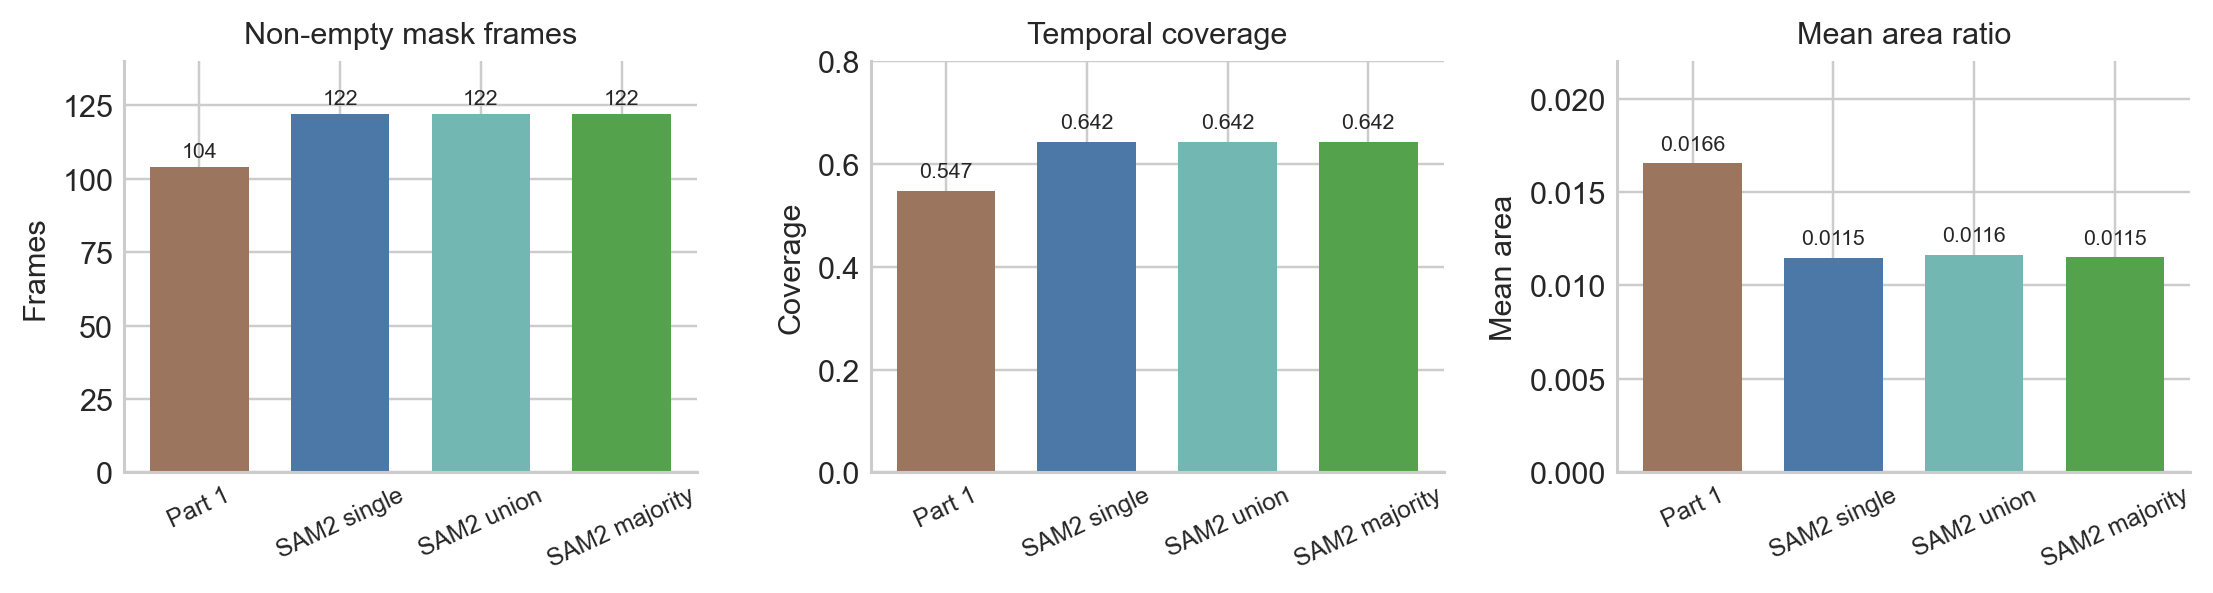
\includegraphics[width=\textwidth]{assets/wild_video2_ablation_metrics.png}
  }{
    \fbox{\rule{0pt}{1.5in}\rule{0.98\textwidth}{0pt}}
  }
  \caption{Quantitative summary of the \texttt{wild\_video2} refinement branches. Single-prompt SAM~2 yields the main improvement over Part 1, while union and majority fusion remain nearly unchanged, confirming that simple prompt ensembling does not materially improve the sequence.}
  \label{fig:wild-ablation-metrics}
\end{figure*}

\subsection{Qualitative Results}
The strongest current qualitative comparisons come from \texttt{bmx-trees} and \texttt{tennis}.
In both cases, keeping the masks fixed and replacing the restoration backend with ProPainter significantly reduces blocky artifacts, transparent ghosting, and inconsistent texture synthesis.
\texttt{wild\_video1} serves as a real-scene success case.
\texttt{wild\_video2} now serves as a failure-to-improvement case: the original Part~2 result shows that weak masks prevent complete removal, while the SAM~2-refined version covers the walking person more consistently and produces a visibly cleaner restoration.
On the same failure case, the lightweight SD2 keyframe baseline produces acceptable single-frame removals, but it does not clearly surpass ProPainter in structure recovery or realism, so we do not treat it as the main extension path.

\begin{figure}[t]
  \centering
  \IfFileExists{assets/bmx_trees_part1_vs_part2.png}{
    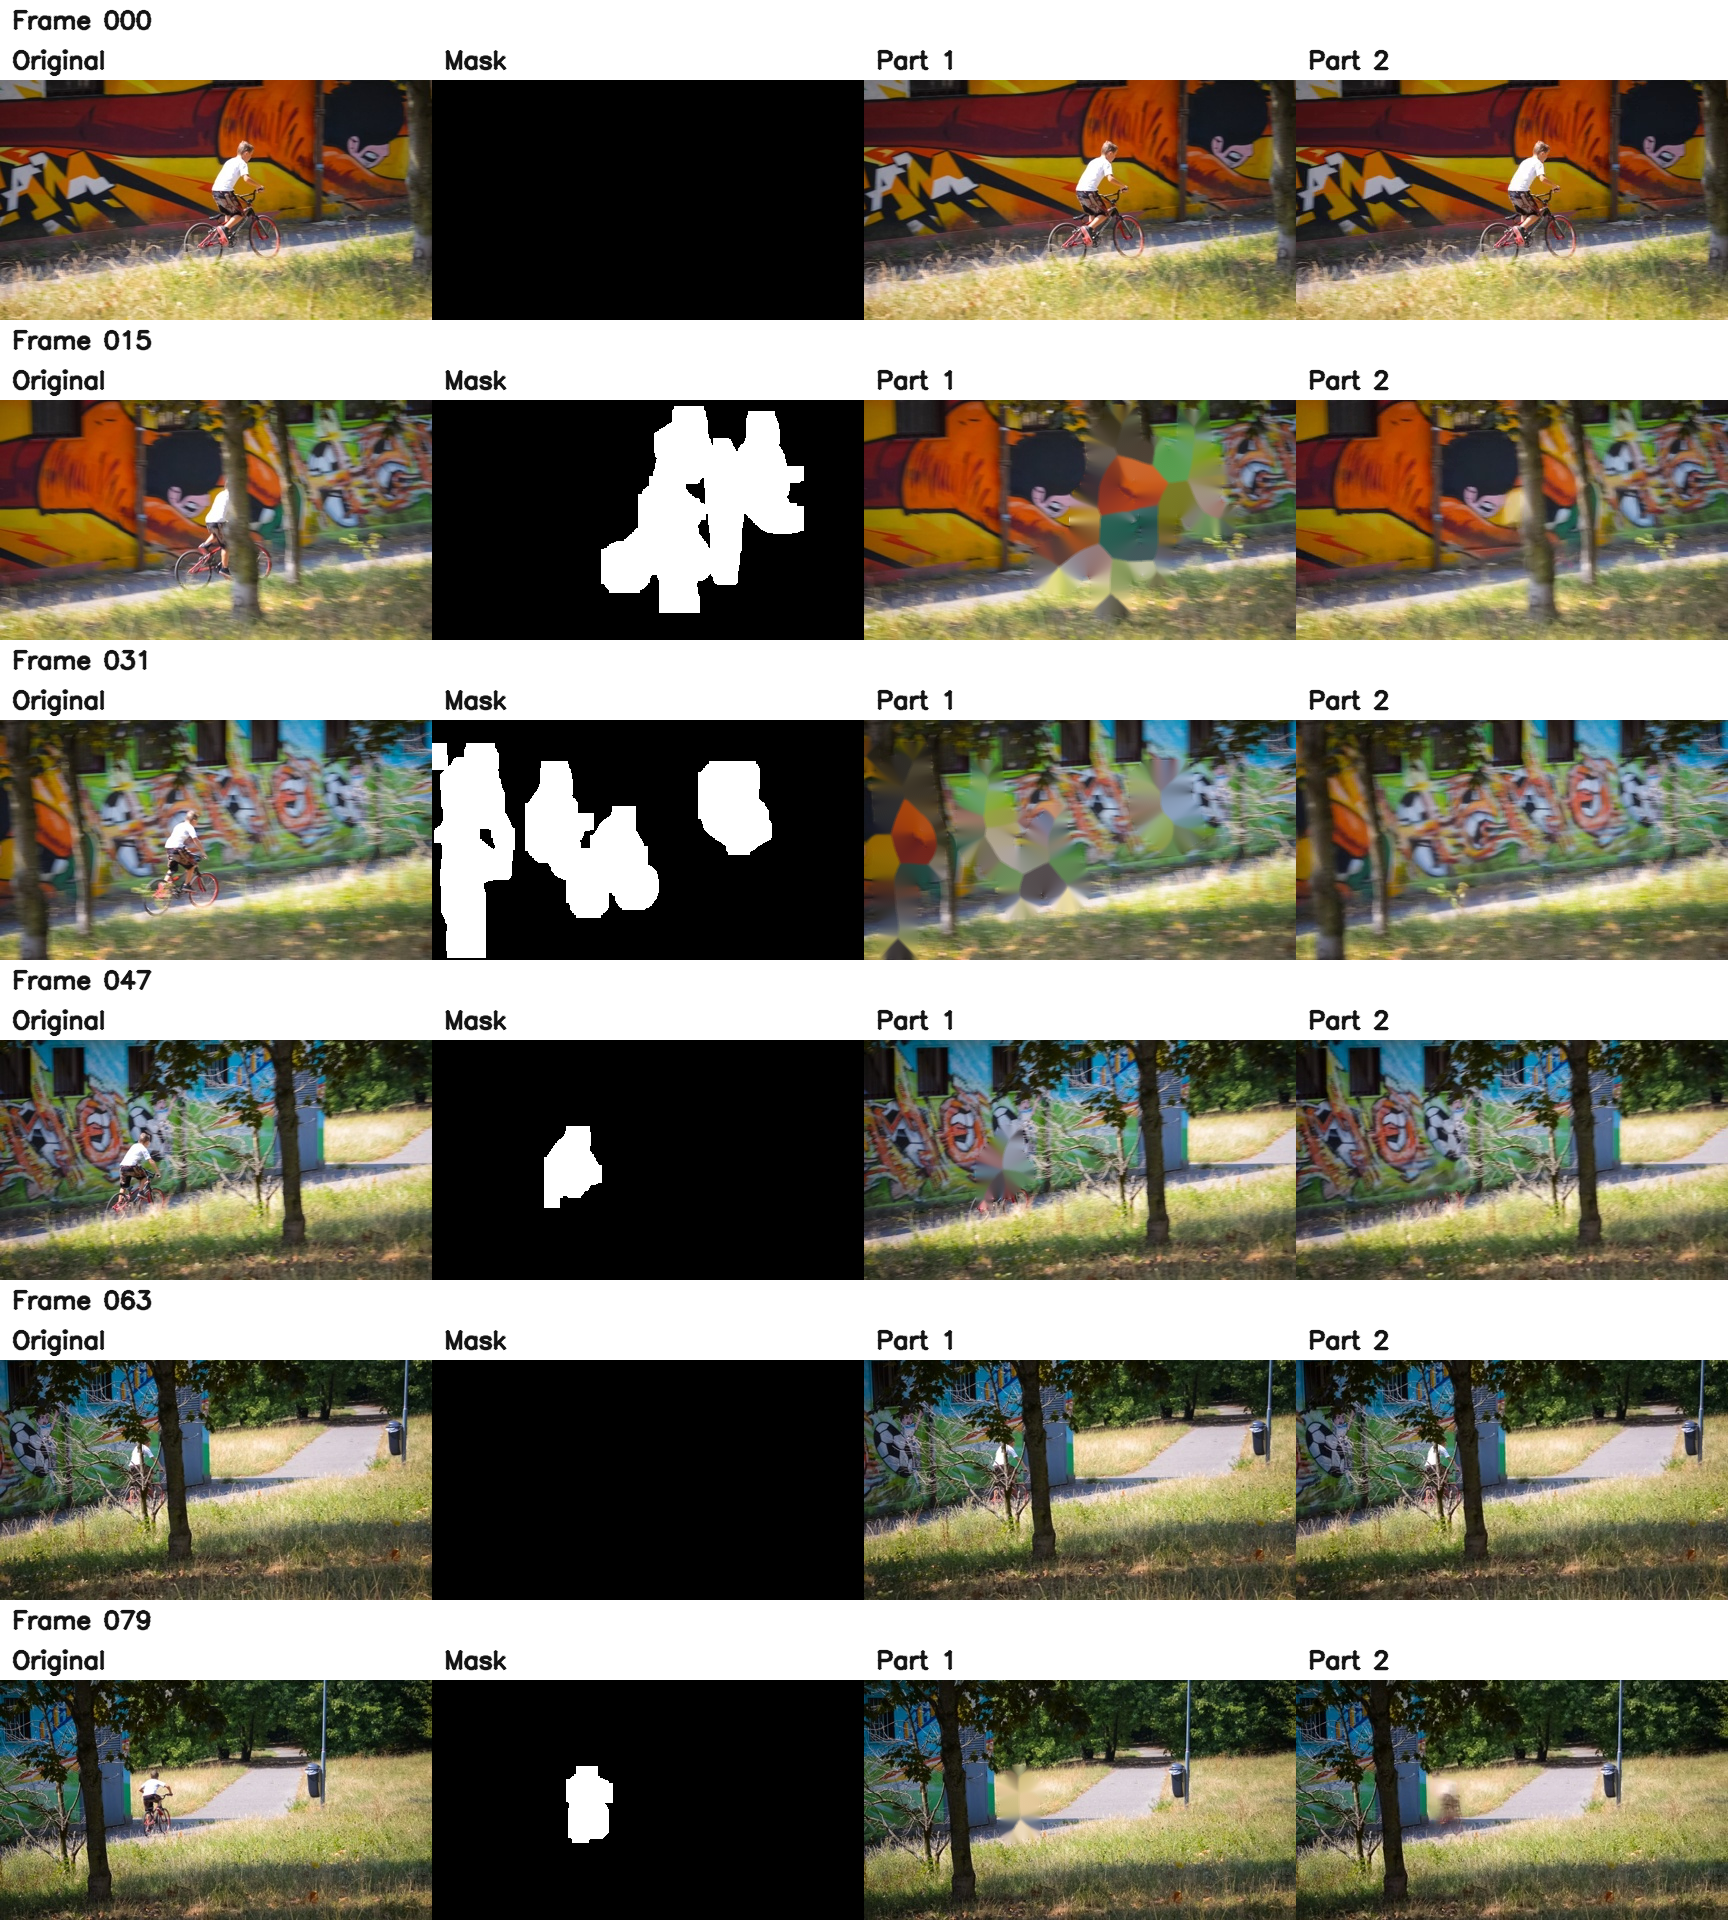
\includegraphics[width=\linewidth]{assets/bmx_trees_part1_vs_part2.png}
  }{
    \fbox{\rule{0pt}{1.2in}\rule{0.95\linewidth}{0pt}}
  }
  \caption{Main qualitative comparison on \texttt{bmx-trees}. Using the same masks, ProPainter produces more coherent background restoration than the classical Part 1 backend.}
\end{figure}

\begin{figure}[t]
  \centering
  \IfFileExists{assets/tennis_part1_vs_part2.png}{
    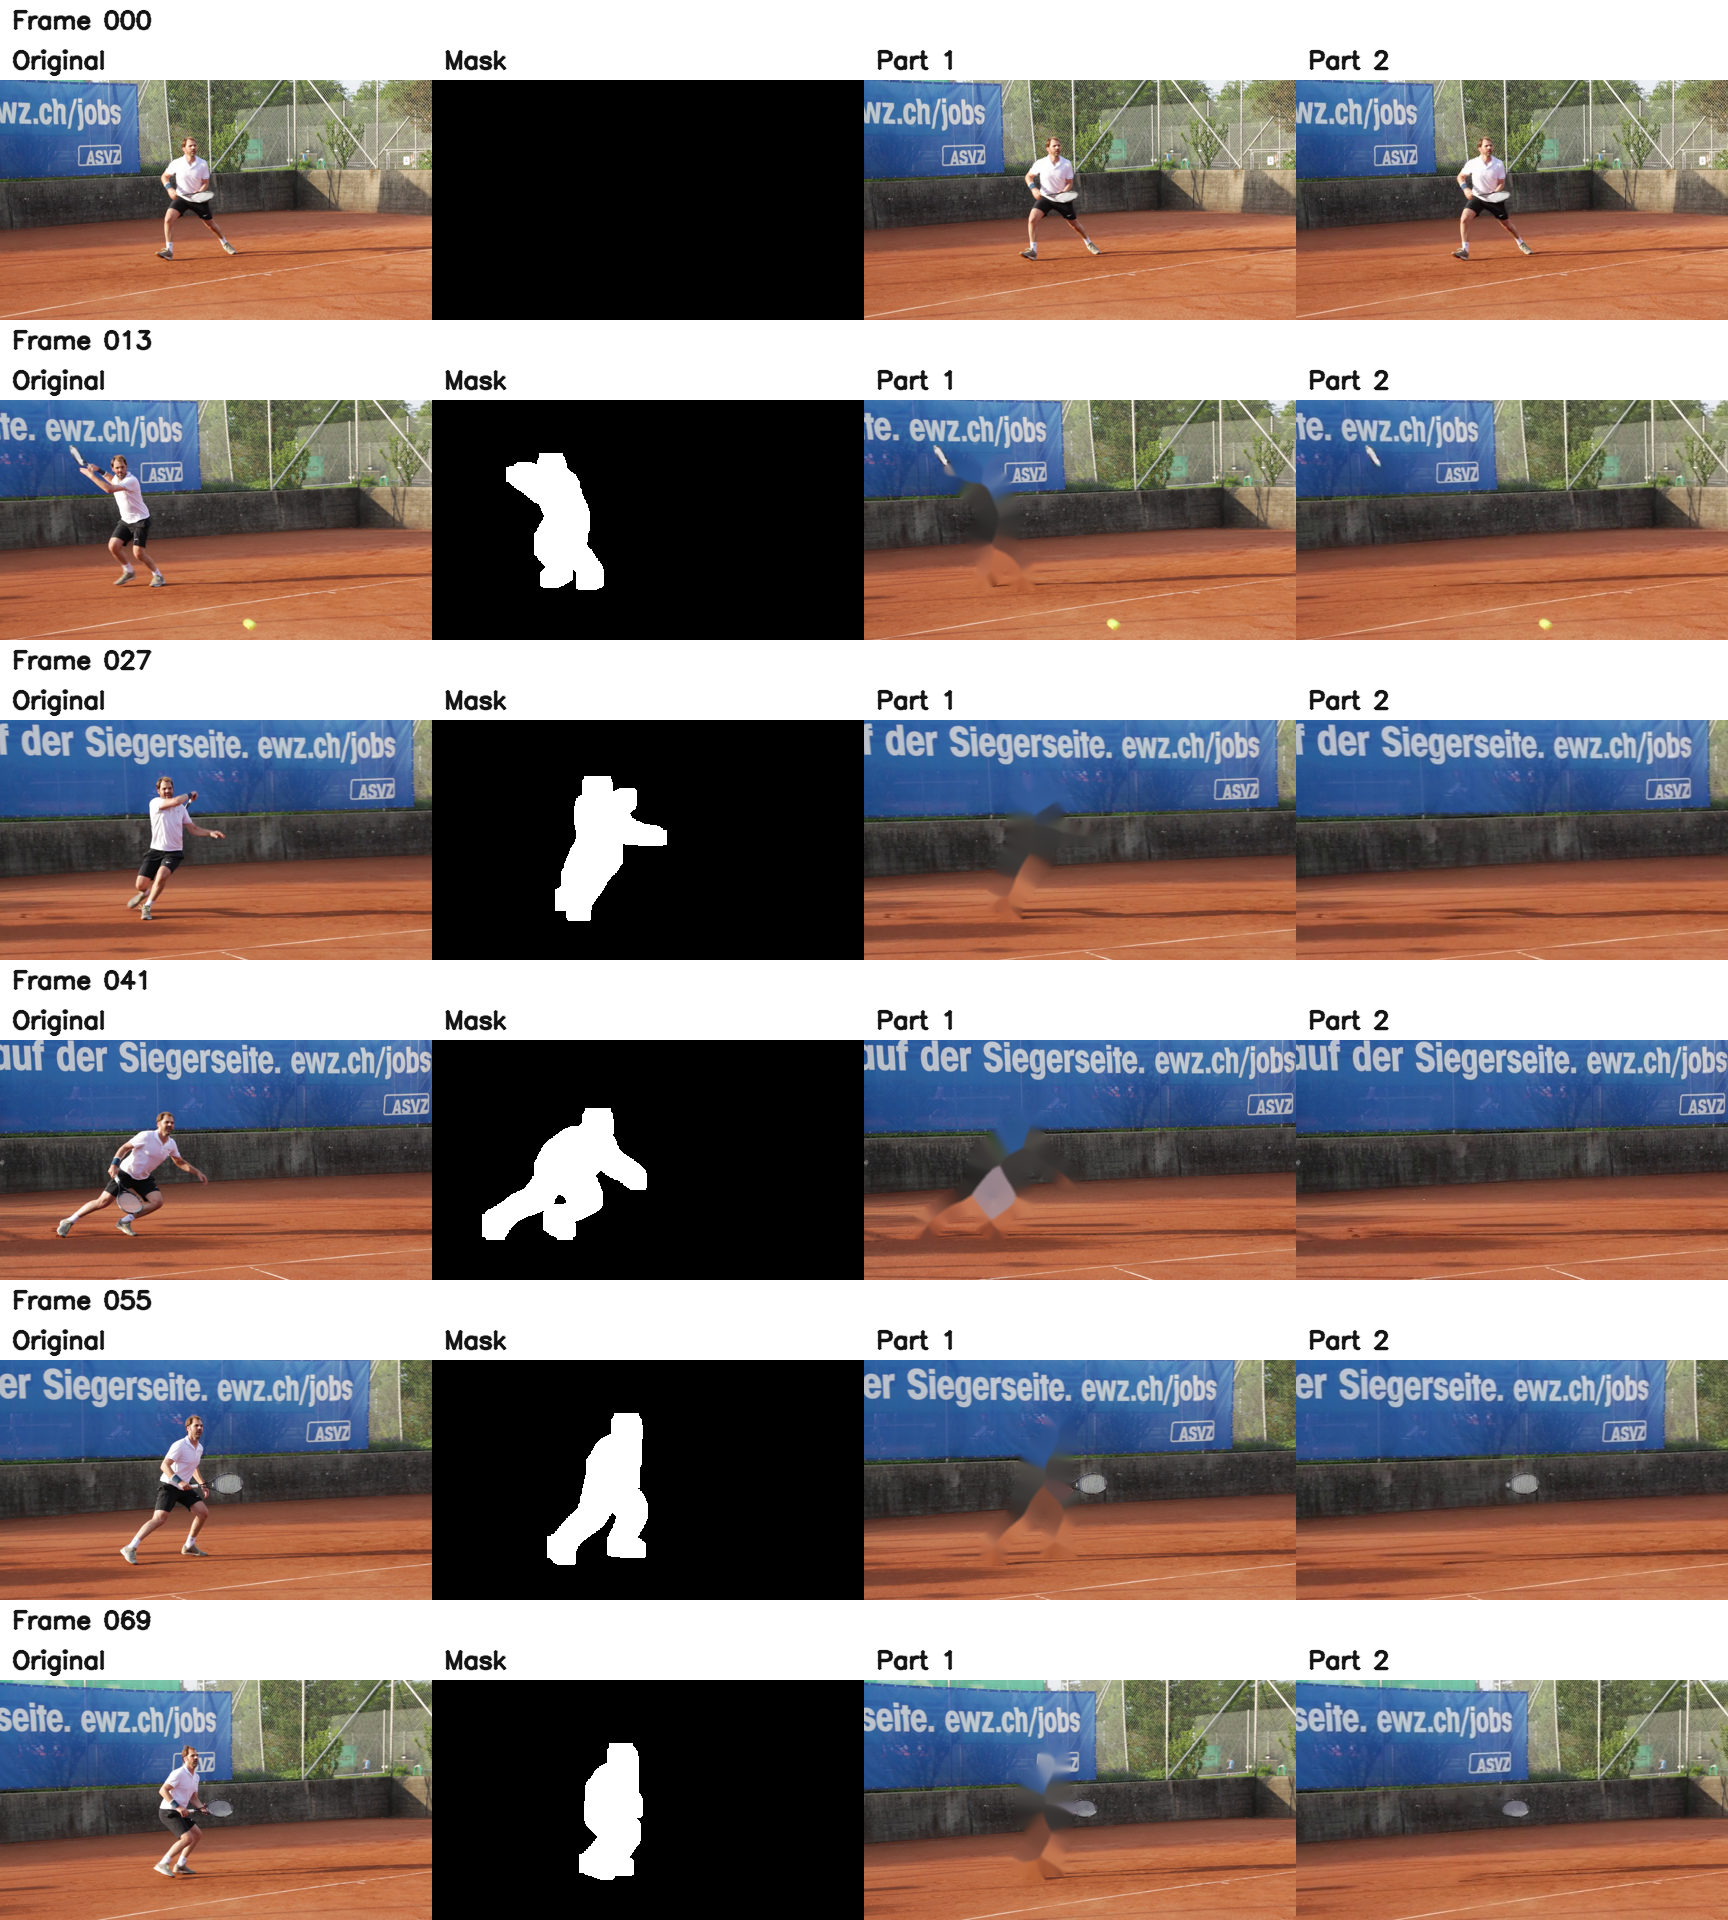
\includegraphics[width=\linewidth]{assets/tennis_part1_vs_part2.png}
  }{
    \fbox{\rule{0pt}{1.2in}\rule{0.95\linewidth}{0pt}}
  }
  \caption{Second controlled comparison on \texttt{tennis}. Even with stronger baseline masks, ProPainter still reduces ghosting and produces cleaner court textures than the Part 1 backend.}
\end{figure}

\begin{figure}[t]
  \centering
  \IfFileExists{assets/wild_video2_part1_vs_sam2_part2.png}{
    \includegraphics[width=\linewidth]{assets/wild_video2_part1_vs_sam2_part2.png}
  }{
    \fbox{\rule{0pt}{1.2in}\rule{0.95\linewidth}{0pt}}
  }
  \caption{Failure-to-improvement case on \texttt{wild\_video2}. Prompt-guided SAM~2 refinement yields better masks and a cleaner final restoration than the original failure case.}
\end{figure}

\subsection{Failure Analysis}
The most important current failure mode is weak mask generation.
In the original \texttt{wild\_video2} setup, the moving person is only partially captured by the baseline mask generator, so both the classical baseline and ProPainter fail to remove the target in missed frames.
After prompt-guided SAM~2 refinement, the masks cover the person more consistently in the key frames and the final restored video is visibly improved, confirming that mask completeness was the main bottleneck in this case.
This interpretation is also supported by the lightweight mask-summary statistics: the refined masks begin slightly earlier, persist later, and remain non-empty for $18$ additional frames compared with the original Part 1 masks.
The multi-prompt ablation sharpens the same conclusion: if the main bottleneck had been prompt-frame selection alone, then fusing several propagation runs would have increased temporal coverage or at least expanded the valid-frame range.
Instead, the merged results remain essentially unchanged.
This suggests that, for this sequence, the decisive improvement is the transition from weak automatic masks to a stronger video-propagation model, while additional prompt ensembling yields only marginal or negligible benefit.
Additional failure modes include overly large masks on thin structures in \texttt{bmx-trees} and residual transparency artifacts in the Part 1 restoration output.
This analysis is important because it clarifies that not all object-removal failures originate from the inpainting network.
In our pipeline, restoration quality depends on both a good completion model and sufficiently accurate masks.
The \texttt{wild\_video2} case therefore acts as a useful diagnostic example: once the mask quality is improved while the restoration backend is held fixed, the final output improves as well.

\section{Discussion and Limitations}
The current project already supports a coherent experimental narrative, but it still has clear limitations.
First, the strongest restoration evidence is qualitative because our wild-video data do not provide clean-background ground truth.
Second, the Part~1 baseline remains sensitive to imperfect detections, especially in scenes with thin structures or large appearance changes.
Third, our SAM~2 refinement experiment is intentionally targeted rather than fully generalized across all sequences.
This is a reasonable design choice for a course project because it produces an interpretable failure analysis, but it does not yet constitute a universal mask-refinement module for every scene.
Fourth, our heavy diffusion-based restoration branch is not complete.
We did finish a lightweight SD2 keyframe baseline on \texttt{wild\_video2}, but the larger SDXL-based AttentiveEraser experiment still requires heavier model deployment.
This distinction matters: the repo now contains completed exploratory diffusion evidence, but not a validated heavy diffusion branch that clearly surpasses ProPainter.

Even with these limitations, the current system is already useful from an experimental standpoint.
The controlled ProPainter comparison demonstrates that the restoration backend matters, while the \texttt{wild\_video2} case demonstrates that better masks can unlock additional gains when restoration is held fixed.
The multi-prompt ablation also improves the honesty of the report: it shows that not every more complicated refinement strategy helps, and that a negative result can still clarify where the real bottleneck lies.
Together, these experiments make the report stronger than a single baseline-only implementation and provide a clear roadmap for future extensions.

\section{Conclusion}
Our current experiments support two clear conclusions.
First, when the removal mask is held fixed, ProPainter provides substantially better restoration quality than the classical temporal median plus \texttt{cv2.inpaint} baseline.
Second, on a real-scene failure case, stronger prompt-guided mask propagation with SAM~2 further improves final object removal quality, confirming that mask quality remains a key bottleneck in the full pipeline.
Third, a simple multi-prompt fusion strategy does not materially outperform the single-prompt SAM~2 result on \texttt{wild\_video2}, which suggests that the main benefit already comes from switching to a stronger propagation model rather than from prompt ensembling.
Fourth, a lightweight SD2 keyframe baseline is feasible but does not clearly outperform ProPainter, so our final recommendation remains a video-level pipeline based on improved masks plus ProPainter rather than a diffusion-first replacement.
Taken together, these results suggest that our project has already moved beyond a single baseline implementation: we now have a reproducible baseline, a controlled Part 1 versus Part 2 comparison, a targeted failure-to-improvement case study, and a small but meaningful ablation that clarifies the limits of our current refinement strategy.
The most natural remaining extensions are to add either more mask-focused evaluation on an annotated subset, a synthetic benchmark for restoration metrics, or a heavier diffusion branch only if a future lightweight baseline demonstrates a more convincing advantage.

\bibliographystyle{ieeenat_fullname}
\bibliography{references}

\end{document}
